\documentclass[tikz,border=8pt]{standalone}
\usepackage{amsmath,amssymb}
\usetikzlibrary{arrows.meta,automata,positioning,quotes}
\begin{document}
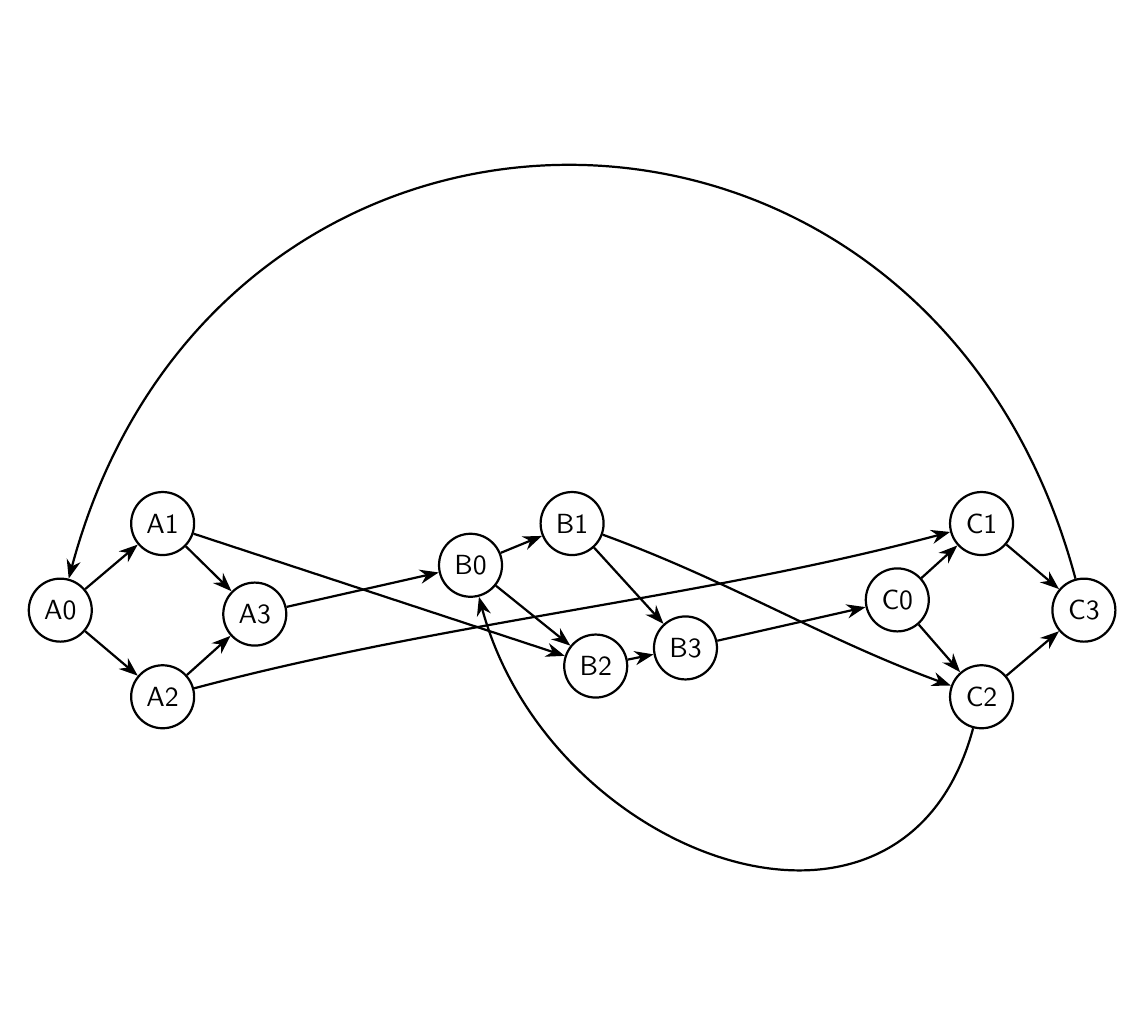
\begin{tikzpicture}[x=1cm,y=1cm]
\tikzset{
  graphnode/.style={circle,draw,thick,minimum size=8mm,inner sep=1pt,font=\sffamily},
  directed/.style={-{Stealth[length=2.4mm]},thick},
  undirected/.style={thick}
}
\node[graphnode] (n_A0) at (0.00,0.00) {A0};
\node[graphnode] (n_A1) at (1.30,1.10) {A1};
\node[graphnode] (n_A2) at (1.30,-1.10) {A2};
\node[graphnode] (n_A3) at (2.47,-0.05) {A3};
\node[graphnode] (n_B0) at (5.21,0.57) {B0};
\node[graphnode] (n_B1) at (6.50,1.10) {B1};
\node[graphnode] (n_B2) at (6.80,-0.71) {B2};
\node[graphnode] (n_B3) at (7.94,-0.48) {B3};
\node[graphnode] (n_C0) at (10.63,0.13) {C0};
\node[graphnode] (n_C1) at (11.70,1.10) {C1};
\node[graphnode] (n_C2) at (11.70,-1.10) {C2};
\node[graphnode] (n_C3) at (13.00,0.00) {C3};
\draw[directed] (n_A0) -- (n_A1);
\draw[directed] (n_A0) -- (n_A2);
\draw[directed] (n_A1) -- (n_A3);
\draw[directed] (n_A2) -- (n_A3);
\draw[directed] (n_B0) -- (n_B1);
\draw[directed] (n_B0) -- (n_B2);
\draw[directed] (n_B1) -- (n_B3);
\draw[directed] (n_B2) -- (n_B3);
\draw[directed] (n_C0) -- (n_C1);
\draw[directed] (n_C0) -- (n_C2);
\draw[directed] (n_C1) -- (n_C3);
\draw[directed] (n_C2) -- (n_C3);
\draw[directed] (n_A3) -- (n_B0);
\draw[directed] (n_B3) -- (n_C0);
\draw[directed] (n_A1) -- (n_B2);
\draw[directed] (n_A2) to[out=15,in=195,looseness=0.85] (n_C1);
\draw[directed] (n_B1) to[out=-20,in=160,looseness=0.9] (n_C2);
\draw[directed] (n_C3) to[dashed,out=105,in=75,looseness=1.45] (n_A0);
\draw[directed] (n_C2) to[dashed,out=-105,in=-75,looseness=1.35] (n_B0);
\end{tikzpicture}
\end{document}
